\begin{figure}[htp]
	\centering
	\subfloat[Initial Noisy Data \newline
		\(\snr{z} = \SI{0.32}{\dB}\)]
	{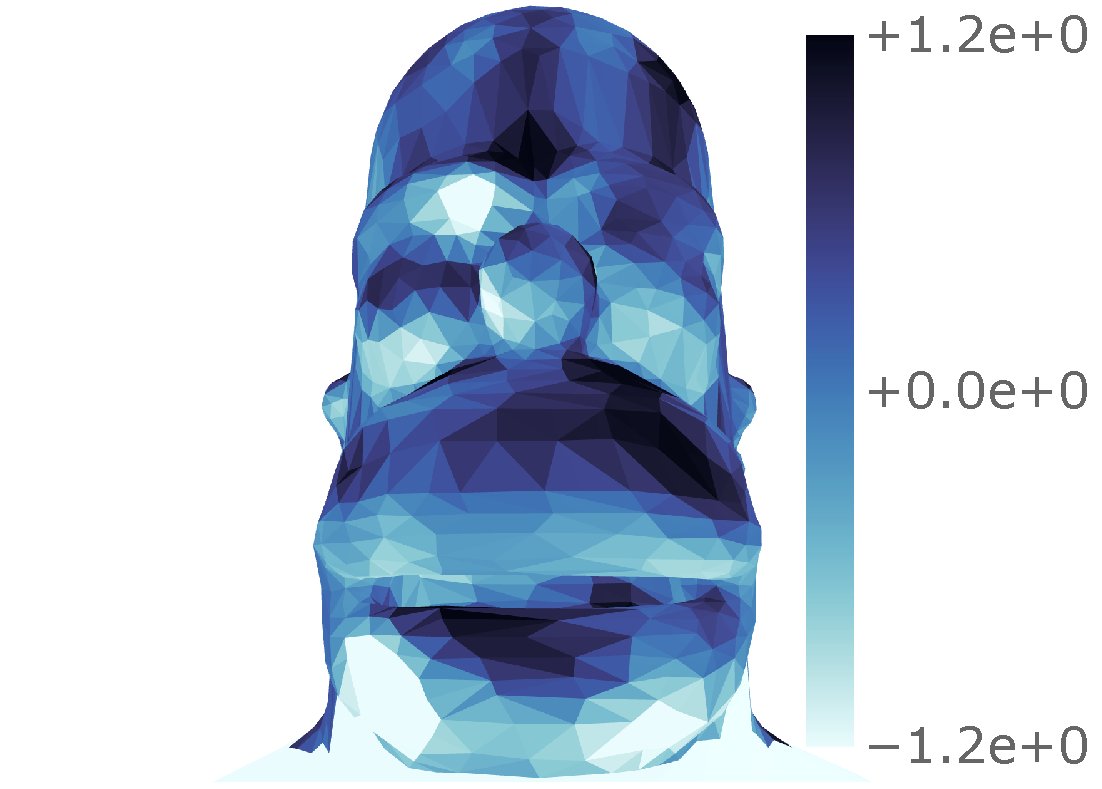
\includegraphics[trim={101 0 3 3},clip,width=.33\textwidth]{slepian_homer_field_-5noise_zoom.pdf}}
	\hfill
	\subfloat[Denoised \(N_{\sigma}=1\) \newline
		\(\snr{d} = \SI{2.29}{\dB}\)]
	{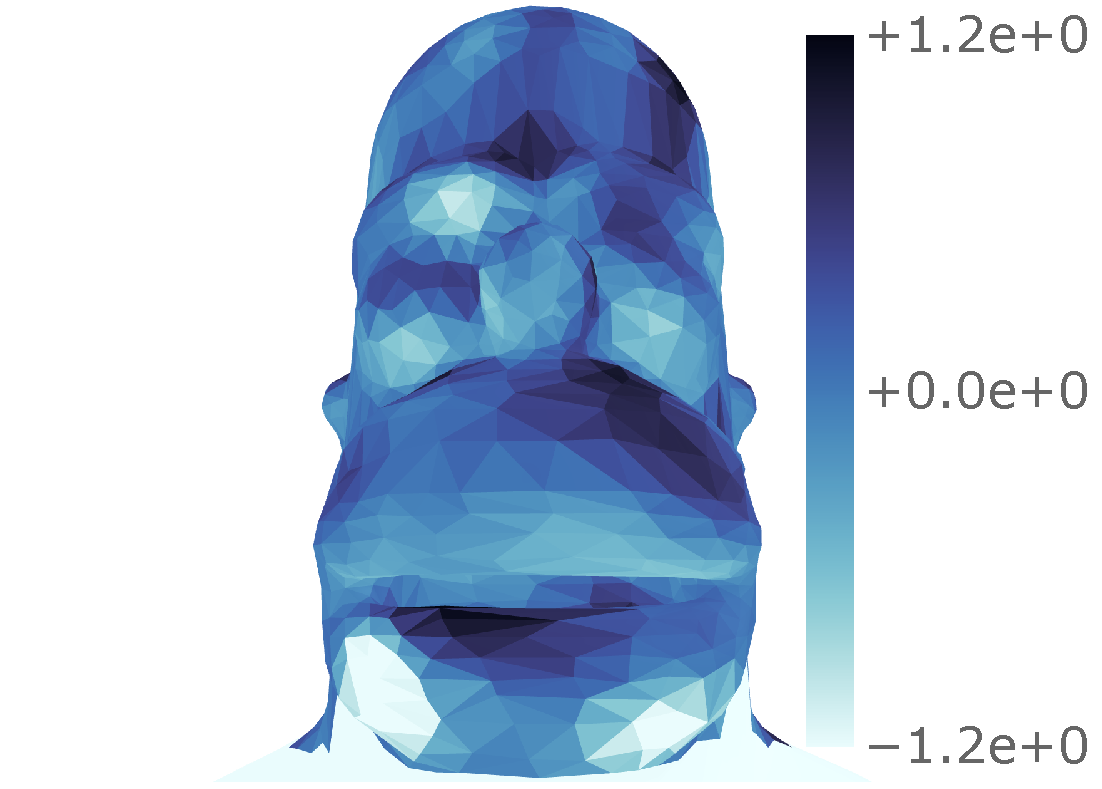
\includegraphics[trim={101 0 3 3},clip,width=.33\textwidth]{homer_-5snr_1n_denoised.pdf}}
	\hfill
	\subfloat[Denoised \(N_{\sigma}=2\) \newline
		\(\snr{d} = \SI{0.98}{\dB}\)]
	{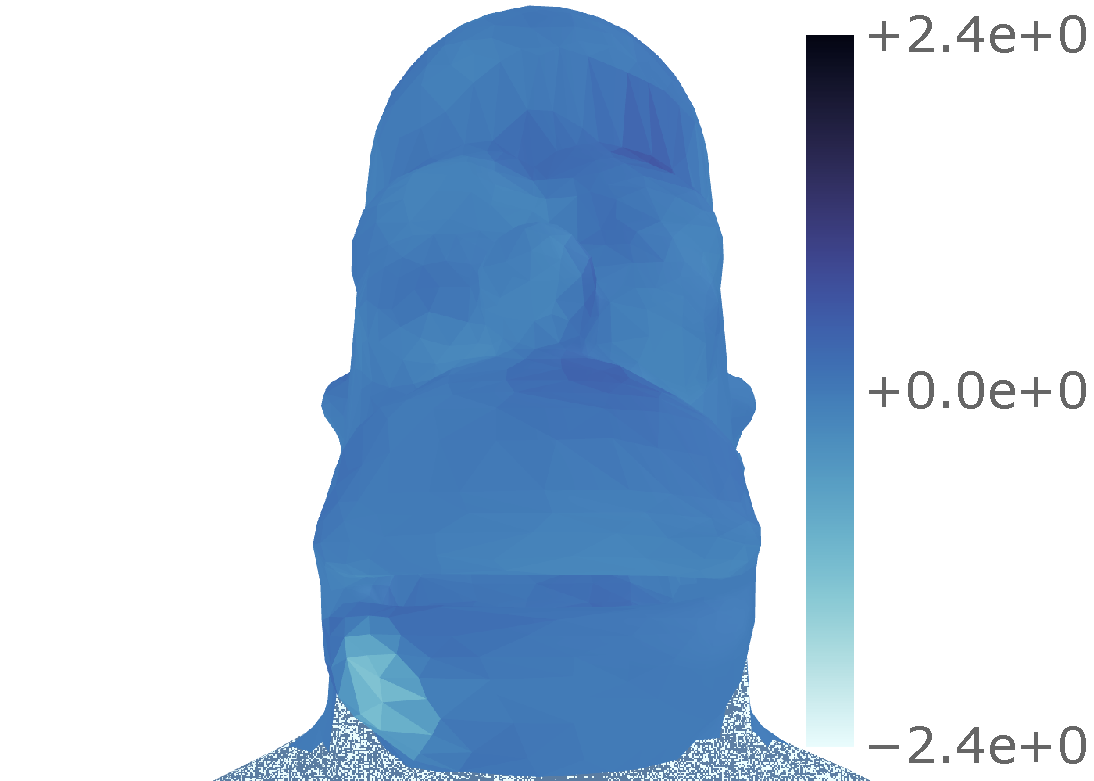
\includegraphics[trim={101 0 3 3},clip,width=.33\textwidth]{homer_-5snr_2n_denoised.pdf}}
	\caption{
		Panel (a) shows the initial noisy signal of the Homer head region with a signal-to-noise ratio of \(\SI{0.32}{\dB}\).
		The scaling and wavelet coefficients of the noisy signal are calculated and are then hard-thresholded for some \(N_{\sigma}\) values.
		The corresponding denoised plots for \(N_{\sigma} \in \set{1, 2}\) are shown in panels (b-c).
		At \(N_{\sigma}=1\) the signal-to-noise ratio is boosted by \(\SI{1.97}{\dB}\) to \(\SI{2.29}{\dB}\).
		As more signal is removed the signal-to-noise ratio decreases to \(\SI{0.98}{\dB}\) at \(N_{\sigma}=2\), which is still higher than the initial noisy signal.
	}\label{fig:chapter4_denoising}
\end{figure}
